\documentclass[aspectratio=169,10pt]{beamer}
\usetheme[progressbar=frametitle,numbering=fraction]{metropolis}
\usepackage[spanish,es-noshorthands]{babel}
\usepackage[utf8]{inputenc}
\usepackage{amsmath,booktabs}
\graphicspath{{../figuras/}}
\setbeamertemplate{frame footer}{Proyecto 2 --- BTYD}
\newcommand{\pvivo}{\mathbb{P}(\text{vivo})}

\title{Contando clientes con modelos \textit{Buy 'Til You Die}}
\subtitle{BG/NBD desde cero: derivación, estimación, pronóstico y sus límites}
\author{Análisis y Ciencia de Datos}
\institute{Facultad de Ingeniería, Universidad del Istmo de Guatemala}
\date{29 de octubre de 2026}

\begin{document}
\maketitle

\begin{frame}{La pregunta}
\begin{itemize}
  \item Contexto \alert{no contractual}: una tienda no ve cuándo se va un cliente.
  \item El gerente quiere saber: ¿cuántas compras harán mis clientes? ¿quiénes siguen ``vivos''?
  \item Los BTYD responden con solo tres números por cliente: \alert{$x$} (frecuencia), \alert{$t_x$} (recencia) y \alert{$T$} (edad).
  \item BTYD es una \emph{familia}: proceso de compra + proceso de muerte + heterogeneidad (+ gasto). El BG/NBD es una elección.
\end{itemize}
\vspace{1em}
\begin{tabular}{lll}\toprule
Modelo & Compra & Muerte\\\midrule
Pareto/NBD & Poisson, $\lambda\sim$ Gamma & cualquier momento\\
\alert{BG/NBD} & Poisson, $\lambda\sim$ Gamma & justo después de cada recompra, $p\sim$ Beta\\
MBG/NBD & Poisson, $\lambda\sim$ Gamma & también tras la primera compra\\\bottomrule
\end{tabular}
\end{frame}

\begin{frame}{Datos: CDNOW (Fader, Hardie y Lee, 2005)}
\begin{columns}[T]
\column{0.38\textwidth}
\begin{itemize}\small
  \item 2{,}357 clientes, primera compra en Q1-1997; 6{,}919 registros $\to$ 6{,}696 transacciones cliente-día.
  \item Calibración: 39 semanas (al 30-sep-1997). \emph{Holdout}: 39 semanas.
  \item \alert{59.9\%} no recompra en calibración.
  \item $T\in[27,\,38.9]$: la cohorte se adquirió escalonadamente, pero la calibración termina igual para todos.
\end{itemize}
\column{0.62\textwidth}
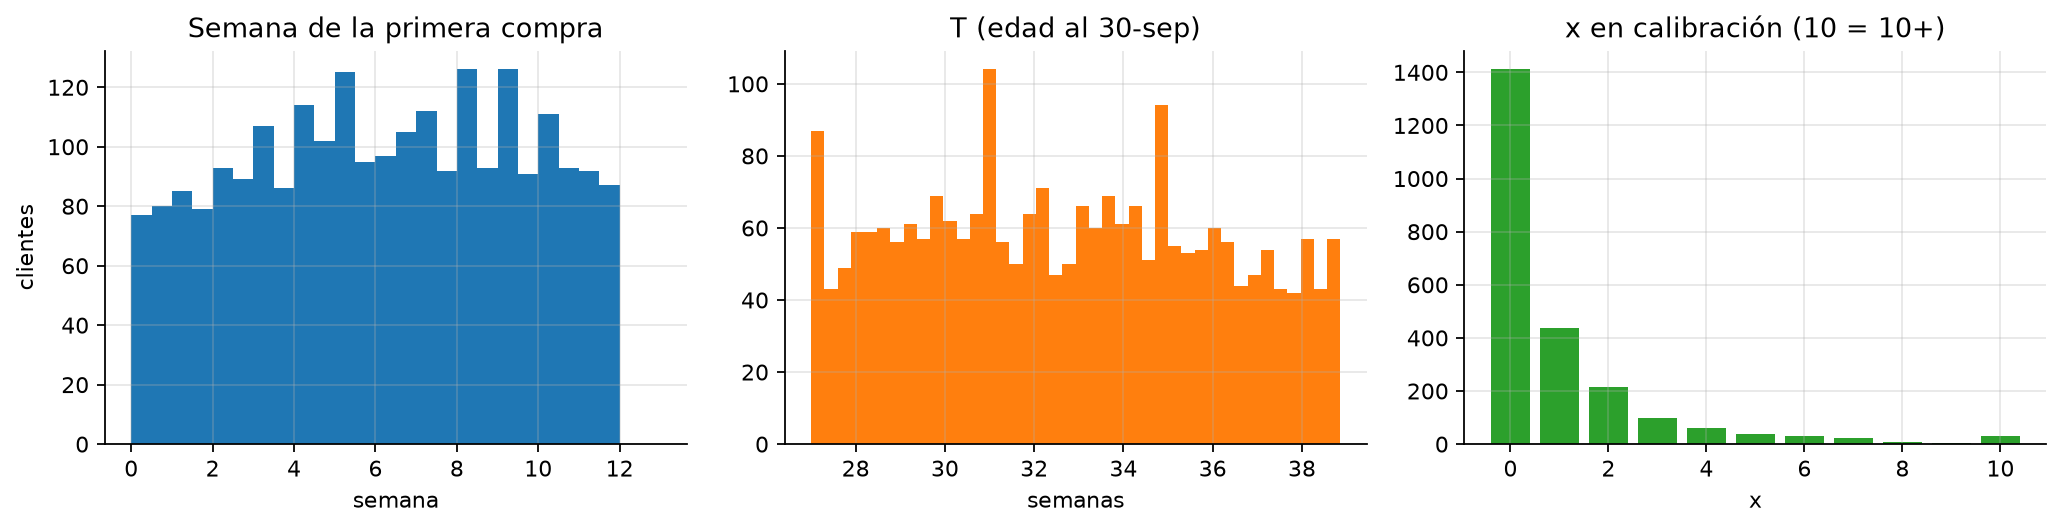
\includegraphics[width=\linewidth]{00_datos}
\end{columns}
\end{frame}

\section{Parte 1: el modelo, pieza por pieza}

\begin{frame}{1.1 Un cliente: dos historias}
Con $\lambda,p$ conocidos, la densidad de $x$ compras Poisson es $\lambda^x e^{-\lambda t_x}$.
\begin{itemize}
  \item \textbf{Vivo en $T$:} sobrevivió $x$ compras y no compró en $(t_x,T]$: $(1-p)^x\lambda^xe^{-\lambda T}$.
  \item \textbf{Murió tras la $x$-ésima:} $p(1-p)^{x-1}\lambda^xe^{-\lambda t_x}$.
\end{itemize}
\[L(\lambda,p\mid x,t_x,T)=(1-p)^x\lambda^xe^{-\lambda T}+\delta_{x>0}\,p(1-p)^{x-1}\lambda^xe^{-\lambda t_x}\]
\alert{Si $x=0$ no hay historia B}: solo se muere justo después de una compra \emph{repetida}. Un cliente sin recompras está vivo por construcción.
\end{frame}

\begin{frame}{1.2 La mezcla}
Integrando $\lambda\sim\text{Gamma}(r,\alpha)$ (mezcla gamma–Poisson) y $p\sim\text{Beta}(a,b)$ (definición de $B$):
\[
L=\frac{\Gamma(r+x)\alpha^r}{\Gamma(r)}\left[\frac{B(a,b+x)}{B(a,b)}\frac{1}{(\alpha+T)^{r+x}}+\delta_{x>0}\frac{B(a+1,b+x-1)}{B(a,b)}\frac{1}{(\alpha+t_x)^{r+x}}\right]
\]
\begin{itemize}
  \item Programada en logaritmos con \texttt{gammaln}, \texttt{betaln}, \texttt{logaddexp}; segundo término solo para $x>0$.
  \item Optimizamos log-parámetros: L-BFGS-B con cotas $\pm10$ desde 6 arranques + Nelder–Mead.
  \item Chequeo: Monte Carlo de la integral de 1.1 coincide con la fórmula (error $<0.04\%$).
  \item Para $x=0$: $L=(\alpha/(\alpha+T))^r$ \alert{no depende de $a,b$}.
\end{itemize}
\end{frame}

\begin{frame}{1.3 ¿Recuperamos parámetros que nosotros pusimos?}
\begin{columns}[T]
\column{0.5\textwidth}\small
$(0.25, 4, 0.8, 2.5)$, 2{,}357 clientes, $T\sim U(27,39)$, \textbf{50 semillas}.\\[0.5em]
\begin{tabular}{lrrr}\toprule
 & media & d.e. & CV\\\midrule
$r$ & 0.254 & 0.010 & 4\%\\
$\alpha$ & 4.05 & 0.27 & 7\%\\
$a$ & 0.86 & 0.20 & 24\%\\
$b$ & 2.75 & 0.73 & 29\%\\
$a/(a+b)$ & 0.241 & 0.018 & 7\%\\\bottomrule
\end{tabular}\\[0.5em]
Sí: sesgo $<$ 0.5 d.e., cobertura 92–96\%.
\column{0.5\textwidth}\small
\textbf{¿Por qué $a,b$ son imprecisos?}
\begin{itemize}
  \item 57\% con $x=0$: \alert{cero información} sobre la muerte.
  \item La muerte se infiere del silencio $T-t_x$, que también puede ser $\lambda$ baja.
  \item corr$(\hat a,\hat b)=0.93$: la \emph{media} de $p$ está bien identificada, su dispersión no.
\end{itemize}
\end{columns}
\vspace{-0.3em}\centering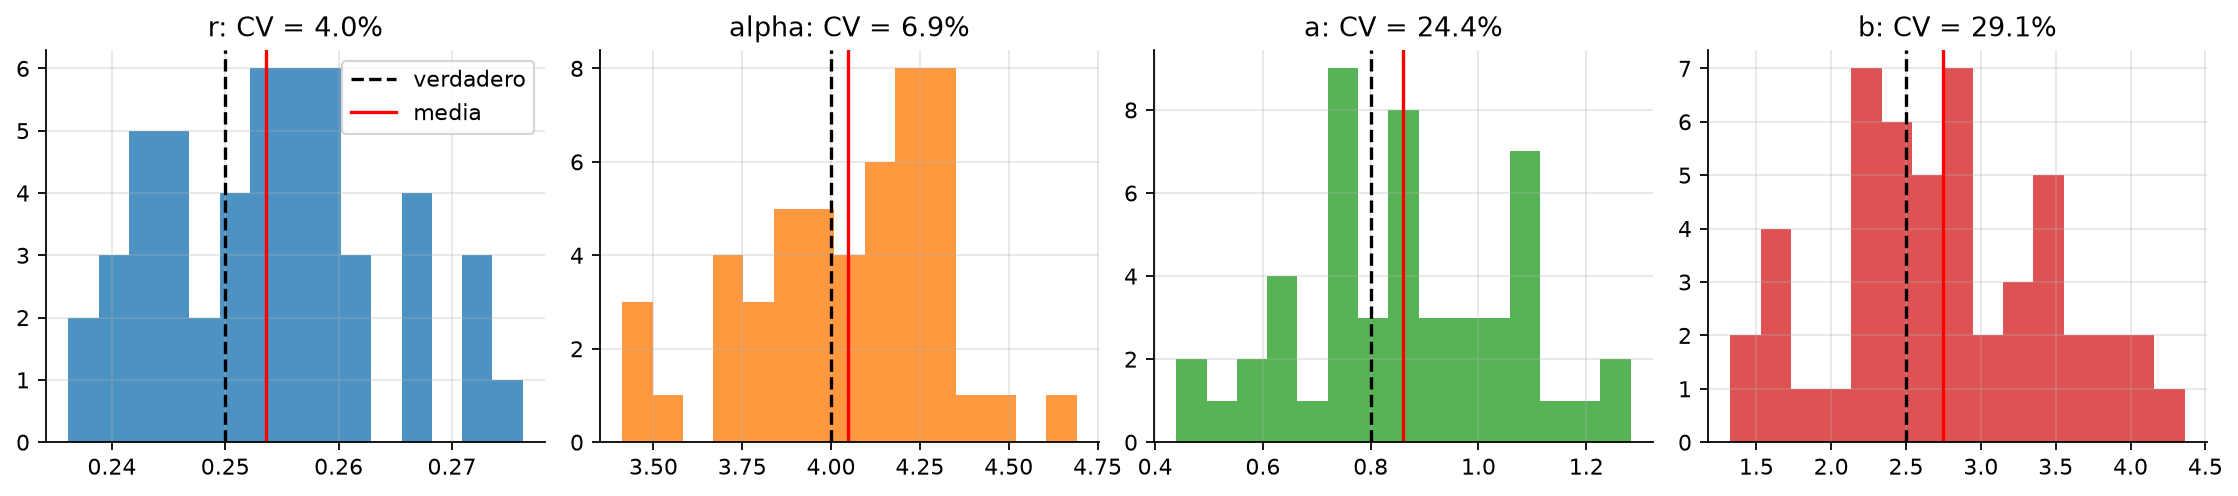
\includegraphics[height=0.27\textheight]{1_3_simulacion}
\end{frame}

\section{Parte 2: ajuste a CDNOW}

\begin{frame}{2.1 Estimados: idénticos al artículo}
\begin{center}
\begin{tabular}{lrrrrr}\toprule
 & $r$ & $\alpha$ & $a$ & $b$ & LL\\\midrule
Nuestro & 0.2426 & 4.4136 & 0.7929 & 2.4259 & $-9582.43$\\
Artículo & 0.243 & 4.414 & 0.793 & 2.426 & $-9582.4$\\
Bootstrap EE & 0.014 & 0.45 & 0.18 & 0.71 & \\\bottomrule
\end{tabular}
\end{center}
\begin{itemize}
  \item Un arranque se perdió en $a\to0$, $b\to\infty$ con LL $=-9763$: \alert{optimizador perdido}, por eso varios arranques.
  \item Bono 2.3: bootstrap (300 réplicas) $\approx$ hessiano $\approx$ simulación para $a,b$; para $\alpha$ el bootstrap es mayor (0.45 vs 0.38): señal de algo de mala especificación en el proceso de compra.
\end{itemize}
\end{frame}

\begin{frame}{2.2 Clientes muy distintos entre sí}
\begin{columns}[T]
\column{0.38\textwidth}\small
\begin{itemize}
  \item $E[\lambda]=r/\alpha=$ \alert{0.055/sem} ($\approx$2.9 recompras/año), pero mediana 0.009: forma de L, CV $=2$.
  \item $E[p]=a/(a+b)=$ \alert{0.246}: uno de cada 4 se va tras cada recompra ($\approx$4 recompras de vida).
  \item $a<1$: muchos muy leales y una cola de ``desertores''.
\end{itemize}
\column{0.62\textwidth}
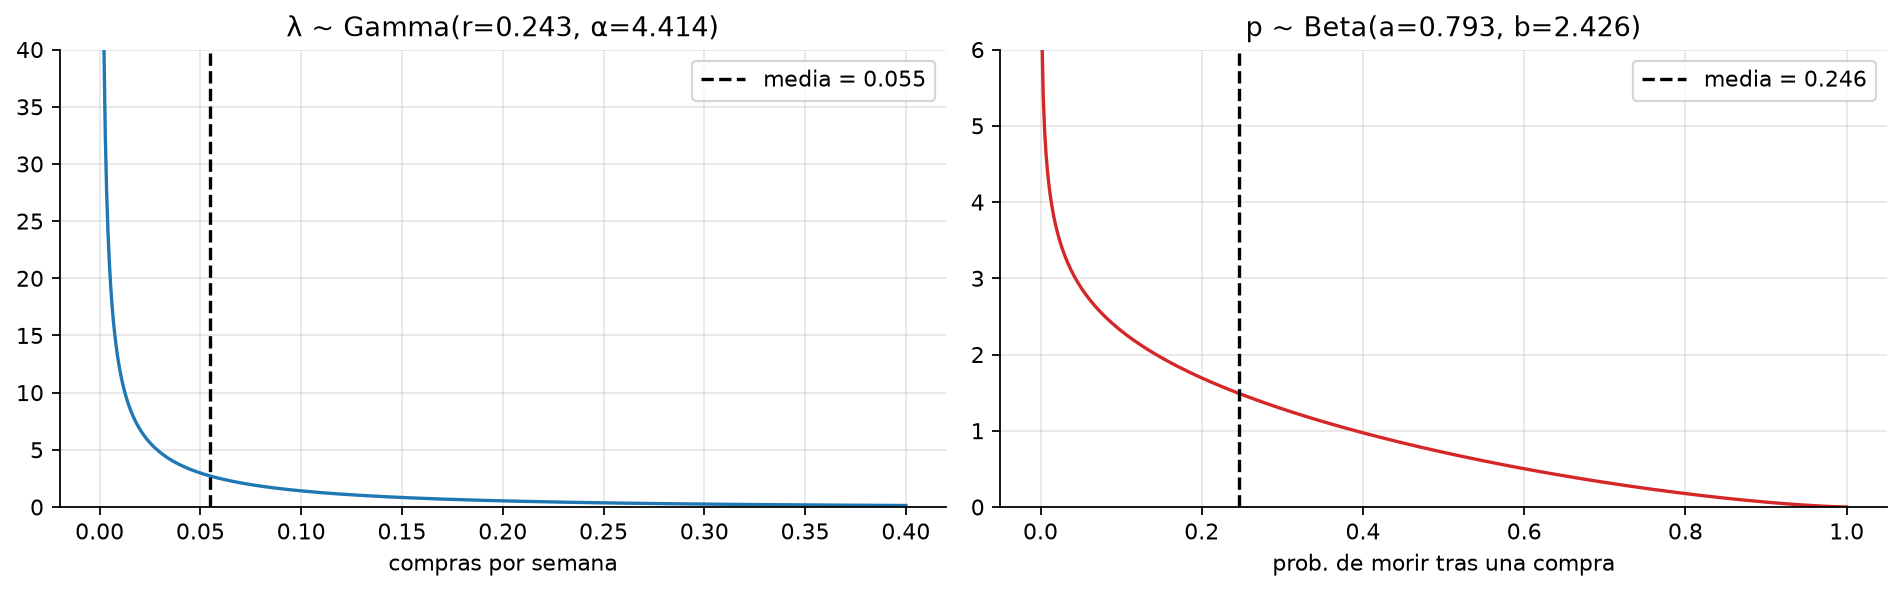
\includegraphics[width=\linewidth]{2_2_densidades}
\end{columns}
\end{frame}

\section{Parte 3: bottom-up vs top-down}

\begin{frame}{3.1 Bottom-up: $\sum_i E[X(t-s_i)]$}
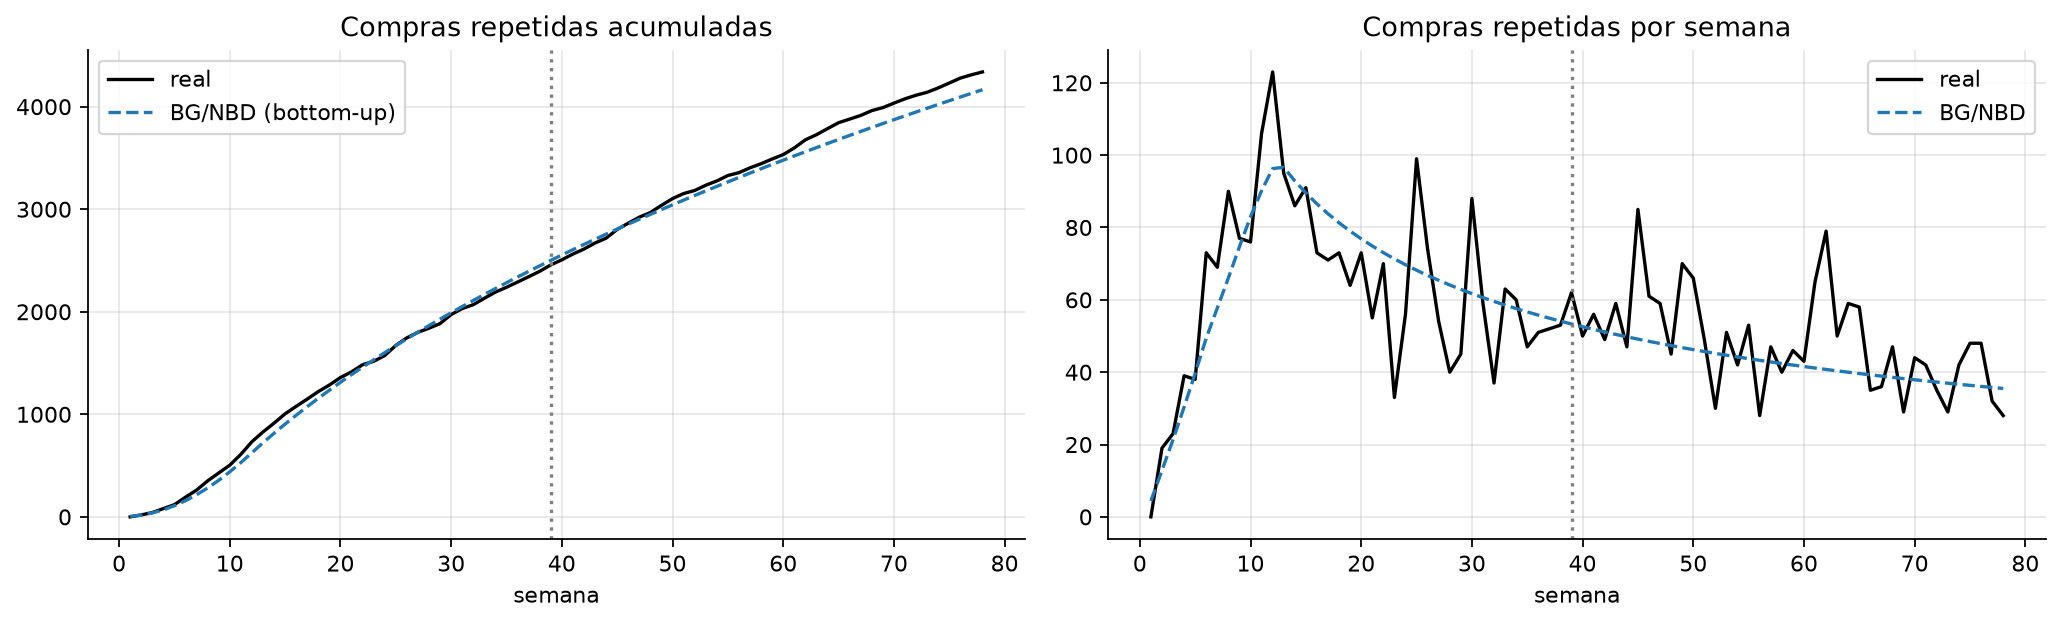
\includegraphics[width=\linewidth]{3_1_bottom_up}
\small Semana 78: 4{,}166 pronosticadas vs 4{,}339 reales $\Rightarrow$ \alert{$-4.0\%$, igual que el artículo}. Solo \emph{holdout}: 1{,}664 vs 1{,}882 ($-11.6\%$).
\end{frame}

\begin{frame}{3.2–3.3 Top-down: ¿cuál ventana?}
\begin{columns}[T]
\column{0.58\textwidth}
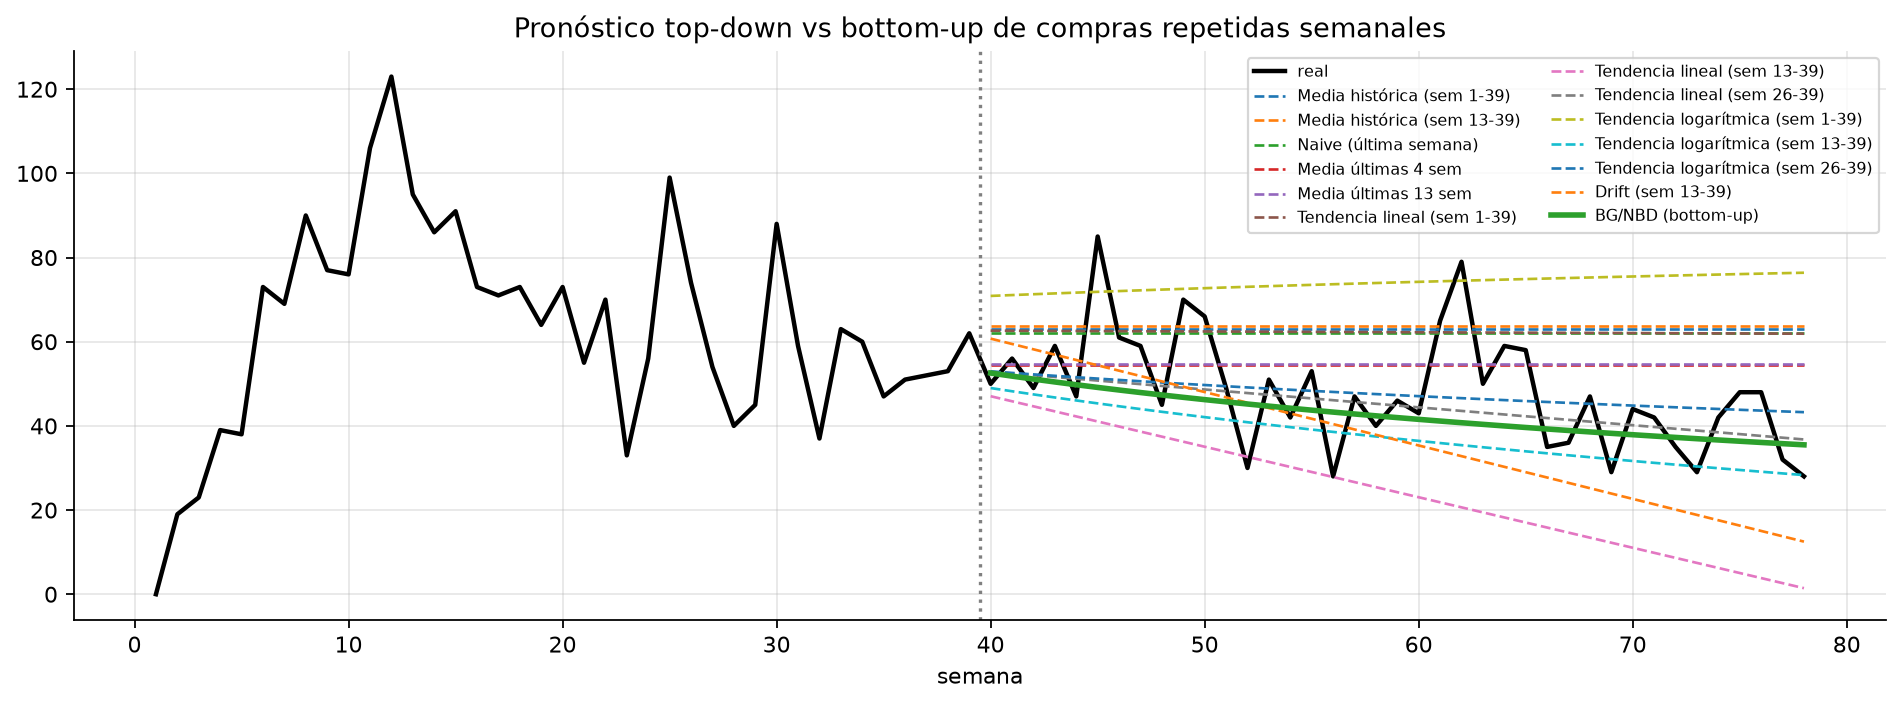
\includegraphics[width=\linewidth]{3_2_top_down}
\column{0.42\textwidth}\scriptsize
\begin{tabular}{lrr}\toprule
Método & error & MAE\\\midrule
Tendencia (26–39) & $-7\%$ & 9.3\\
\alert{BG/NBD} & $-12\%$ & 9.8\\
Media últ. 4 & $+13\%$ & 12.3\\
Media últ. 13 & $+13\%$ & 12.4\\
Drift (13–39) & $-24\%$ & 15.1\\
Naive & $+28\%$ & 16.6\\
Tendencia (1–39) & $+29\%$ & 16.7\\
Media (1–39) & $+31\%$ & 17.3\\
Tendencia (13–39) & $-50\%$ & 24.2\\\bottomrule
\end{tabular}
\end{columns}
\small El ganador ex post depende de la ventana: la misma tendencia va de $-50\%$ a $+29\%$. El BG/NBD no tiene ventanas que escoger.
\end{frame}

\begin{frame}{3.3 Las primeras 12 semanas}
\begin{columns}[T]
\column{0.55\textwidth}
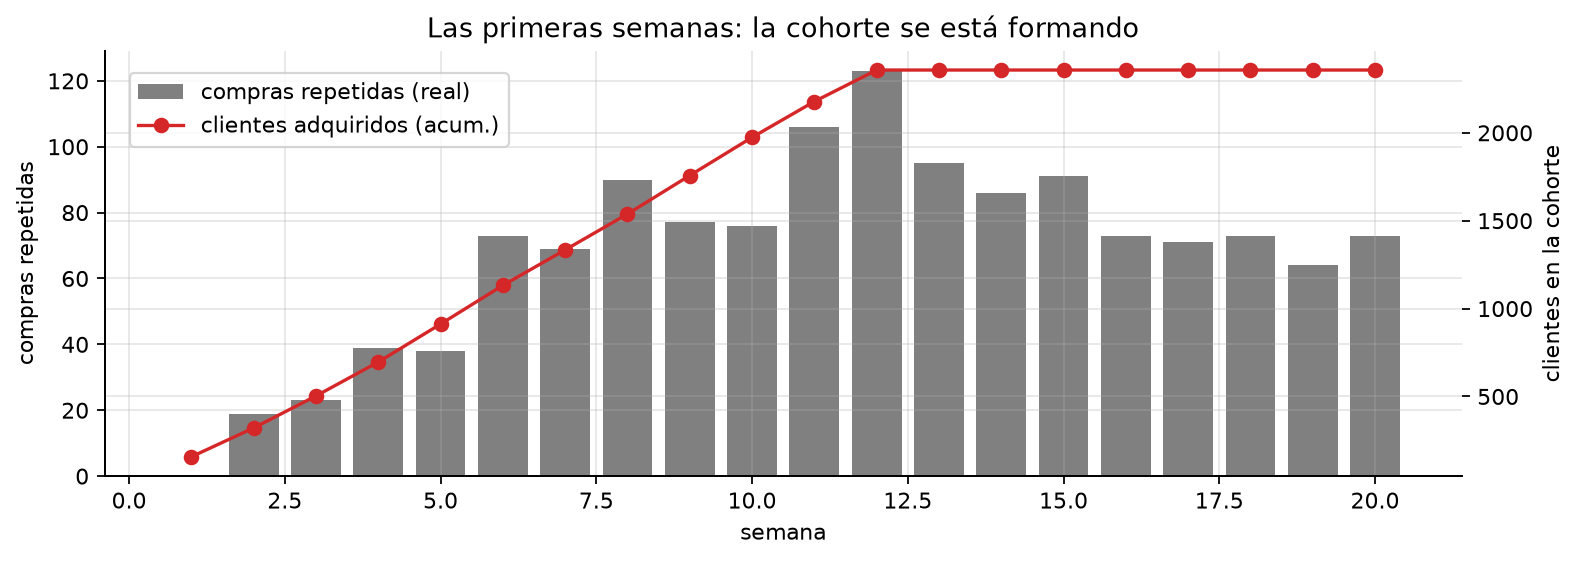
\includegraphics[width=\linewidth]{3_3_primeras_semanas}
\column{0.45\textwidth}
\begin{itemize}
  \item La \alert{cohorte se está formando}: llegan clientes hasta la semana 12, y las recompras suben por pura adquisición.
  \item Desde la 13 la cohorte está cerrada y se va muriendo.
  \item Un top-down solo ve ``sube y baja''; no sabe que la adquisición paró ni cuántos siguen vivos.
\end{itemize}
\end{columns}
\end{frame}

\begin{frame}{3.4 Por cliente: esperanzas condicionales}
\begin{columns}[T]
\column{0.5\textwidth}
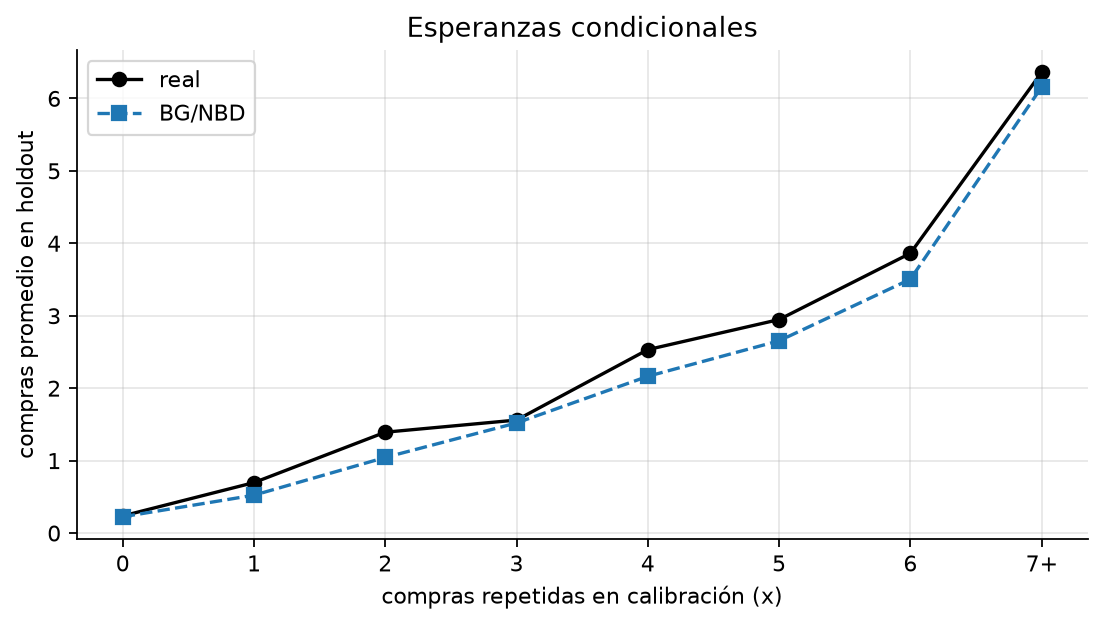
\includegraphics[width=\linewidth]{3_4_condicional}
\column{0.5\textwidth}\small
\begin{itemize}
  \item $x=0$: 0.225 vs 0.237 real (artículo: 0.23 vs 0.24). $x=3$: 1.52 vs 1.56.
  \item Más error en \alert{$x=1,2$ ($-25\%$)}: el modelo mata demasiado pronto a los que recompraron poco.
  \item corr$(x^*,E[Y])=0.626$, como en el artículo.
  \item Un top-down \alert{no puede} hacer esto: no sabe quién compone el total.
\end{itemize}
\end{columns}
\end{frame}

\section{Parte 4: ¿quién sigue vivo?}

\begin{frame}{4.1–4.2 $\pvivo$ como clasificador: peor que una moneda}
\begin{columns}[T]
\column{0.45\textwidth}\small
Tasa base: 29.0\% compra en el \emph{holdout}.\\[0.3em]
\begin{tabular}{lrr}\toprule
 & pred 0 & pred 1\\\midrule
$Z=0$ & 254 & 1419\\
$Z=1$ & 139 & 545\\\bottomrule
\end{tabular}\\[0.3em]
Exactitud 34\% (vs 71\% de ``nadie compra''). \alert{AUC = 0.316}.
\column{0.55\textwidth}\small
\textbf{¿Por qué?}
\begin{itemize}
  \item Con $x=0$, \alert{$\pvivo=1$ exactamente}: sin recompras no hubo oportunidad de morir.
  \item Pero de esos 1{,}411 solo compra el \alert{13.7\%} (vs 51.9\% con $x>0$).
  \item El ranking pone primero, empatados, al grupo que menos compra.
  \item Entre $x>0$, AUC = 0.70.
\end{itemize}
\alert{``Vivo'' no es ``va a comprar''.}
\end{columns}
\end{frame}

\begin{frame}{4.3 La probabilidad correcta}
\begin{enumerate}
  \item En el BG/NBD solo se muere tras comprar $\Rightarrow$ un vivo que no compra sigue vivo: $P(0\text{ en }\tau\mid\lambda)=e^{-\lambda\tau}$.
  \item Posterior: $\lambda\mid\text{vivo}\propto\lambda^{r-1}e^{-\alpha\lambda}\cdot\lambda^xe^{-\lambda T}\Rightarrow\text{Gamma}(r+x,\alpha+T)$.
  \item Gamma–Poisson: $P(0\text{ en }\tau\mid\text{vivo})=\left(\frac{\alpha+T}{\alpha+T+\tau}\right)^{r+x}$.
\end{enumerate}
\[\boxed{\mathbb{P}(Z=1\mid x,t_x,T)=\pvivo\left[1-\left(\frac{\alpha+T}{\alpha+T+\tau}\right)^{r+x}\right]}\]
4.4: verificada por simulación (20 copias de la cohorte): en cada decil fórmula y simulación difieren $<0.013$.
\end{frame}

\begin{frame}{4.5 En datos reales: ¿ordena mejor que una sola variable?}
\begin{columns}[T]
\column{0.62\textwidth}
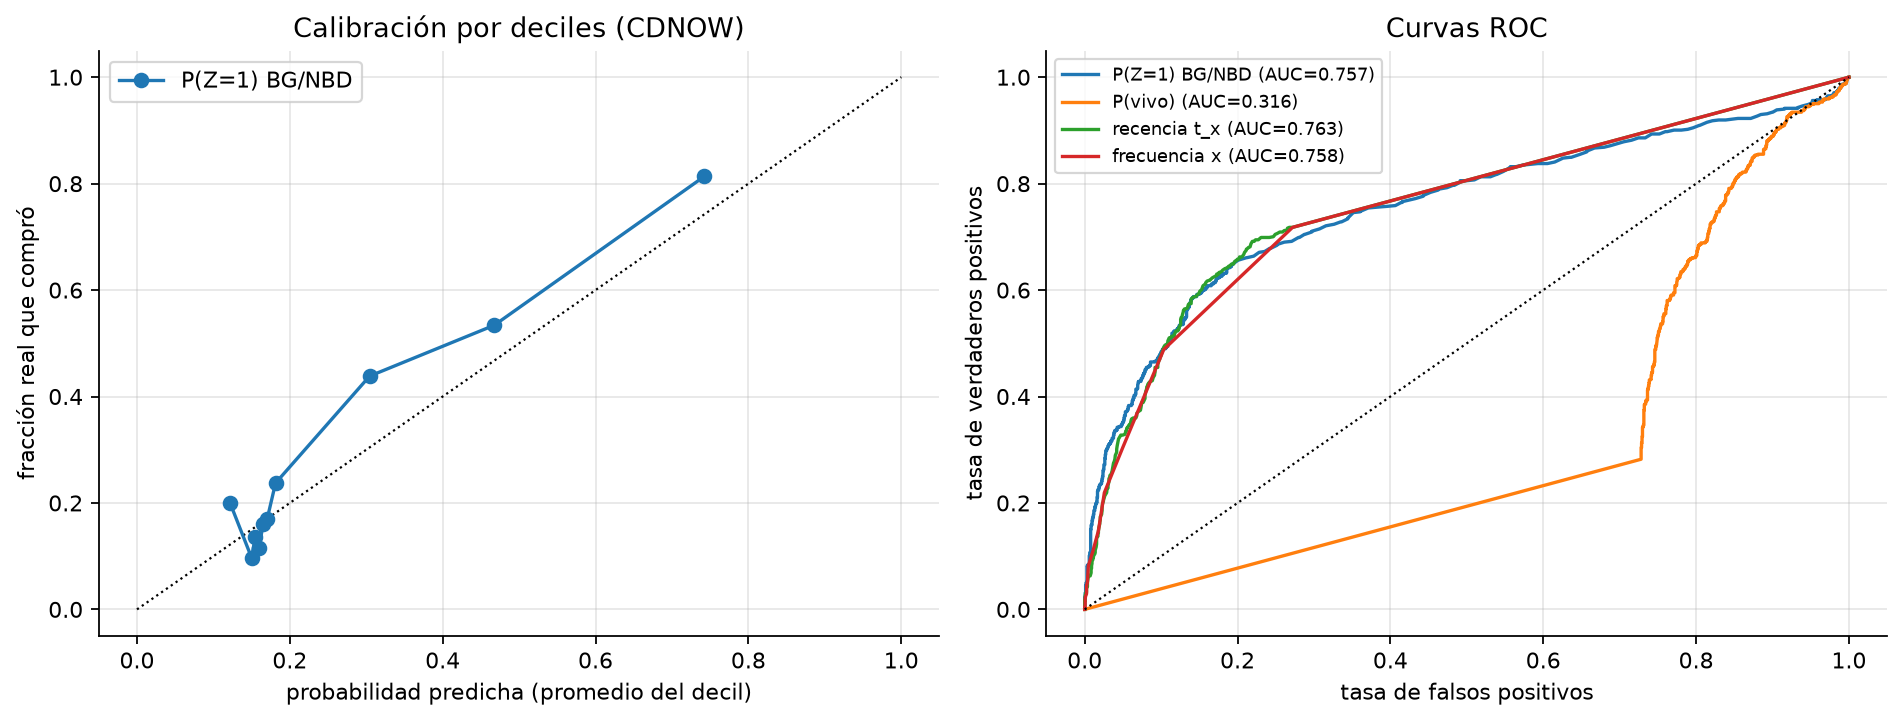
\includegraphics[width=\linewidth]{4_5_calibracion_roc}
\column{0.38\textwidth}\small
\begin{tabular}{lr}\toprule
 & AUC\\\midrule
$P(Z=1)$ & 0.757\\
recencia $t_x$ & 0.763\\
frecuencia $x$ & 0.758\\\bottomrule
\end{tabular}\\[0.3em]
Brier 0.161 vs 0.206 (tasa base).\\[0.3em]
\alert{Honestamente: no ordena mejor que la recencia.} Lo que aporta: probabilidades calibradas, cualquier horizonte, totales y $E[Y]$, sin etiquetas.
\end{columns}
\end{frame}

\begin{frame}{4.6 MBG/NBD: cambiar una pieza}
\begin{columns}[T]
\column{0.55\textwidth}
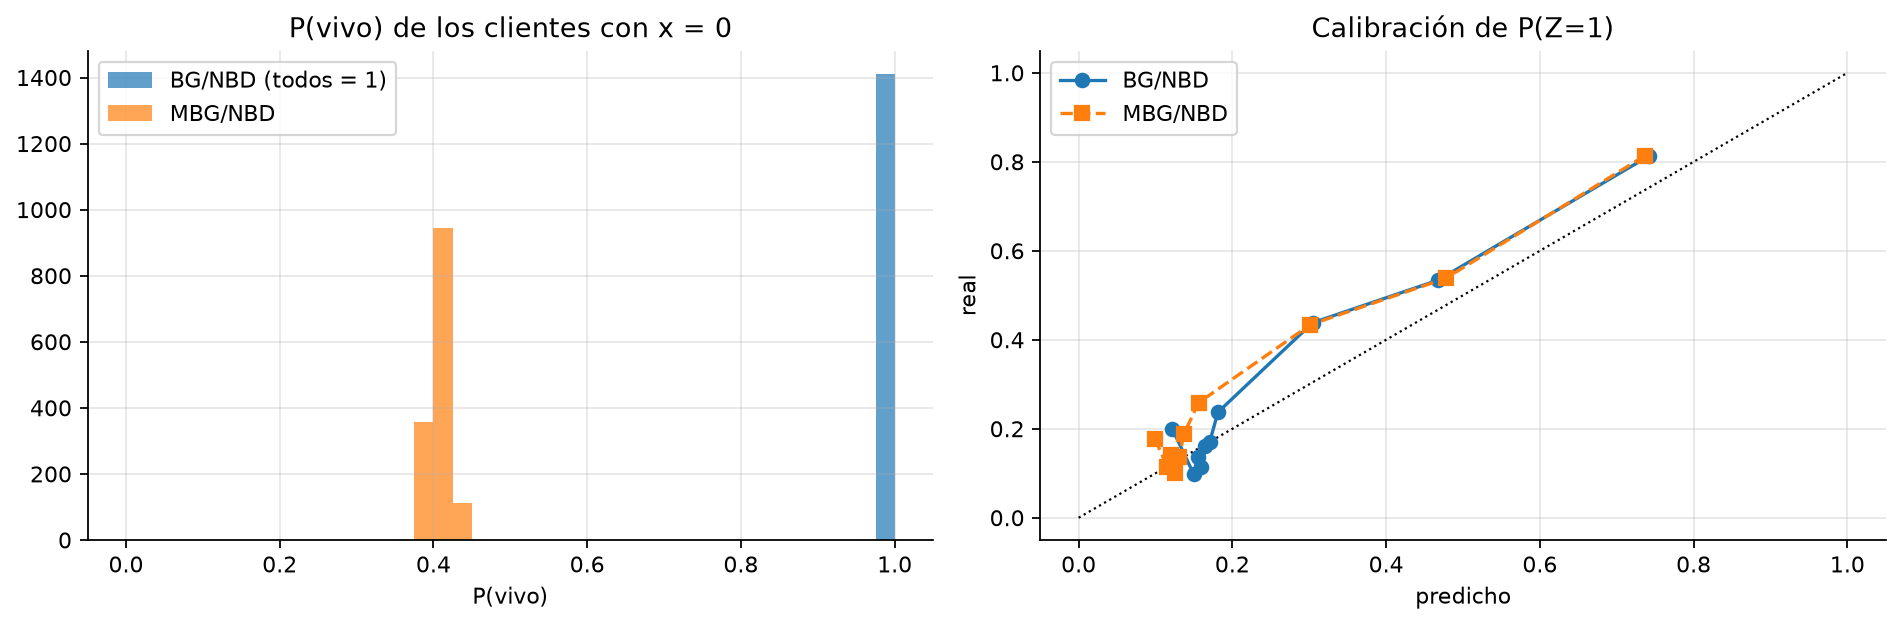
\includegraphics[width=\linewidth]{4_6_mbgnbd}
\column{0.45\textwidth}\scriptsize
\begin{tabular}{lrr}\toprule
 & BG & MBG\\\midrule
LL & $-9582.43$ & $-9582.14$\\
$\pvivo$, $x=0$ & 1.00 & 0.41\\
AUC $\pvivo$ & 0.316 & 0.687\\
AUC $P(Z=1)$ & 0.757 & 0.760\\
Brier & 0.1612 & 0.1614\\
Holdout (real 1882) & 1664 & 1572\\\bottomrule
\end{tabular}\\[0.3em]
\small La fórmula de 4.3 sigue valiendo (muerte solo tras comprar). Para la promoción: ordenan igual (Spearman 0.98); \alert{MBG si se reporta $\pvivo$}, BG para niveles.
\end{columns}
\end{frame}

\section{Parte 5: Online Retail}

\begin{frame}{5.1 Nadie se muere}
\begin{itemize}
  \item 2{,}957 clientes; calibración dic-2010 a jun-2011, \emph{holdout} 23 semanas.
  \item $\hat r=0.74$, $\hat\alpha=9.17$, pero \alert{$\hat a\to0$, $\hat b\to\infty$}: $E[p]\approx10^{-11}$. Mismo LL que el NBD sin muerte ($-15107.235$).
  \item ¿Por qué? \textbf{Mayoristas} que reabastecen; \textbf{silencios cortos} ($T-t_x$ medio 6 vs 16 semanas; solo 8\% con más de medio año callado vs 69\% en CDNOW); \textbf{calibración corta} y ``primeras compras'' que no lo son (30\% aparece en dic-2010: truncamiento por la izquierda, sobrevivientes).
\end{itemize}
\end{frame}

\begin{frame}{5.2 No ve venir noviembre}
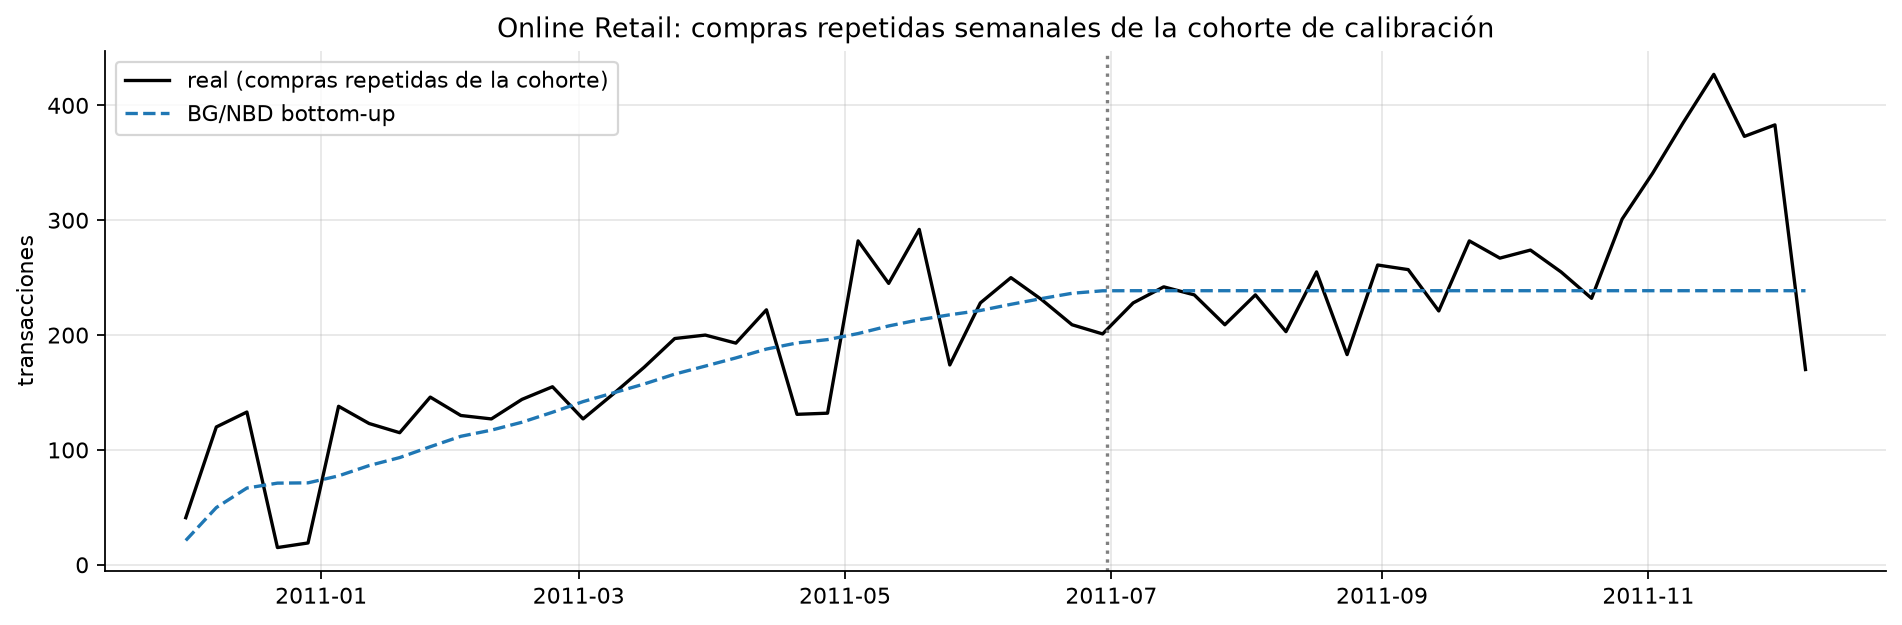
\includegraphics[width=\linewidth]{5_2_online_retail}
\small Holdout: 5{,}489 vs 6{,}313 reales (\alert{$-13\%$}). Jul–ago $+7$–$10\%$; \alert{noviembre $-38\%$}. El BG/NBD supone tasas constantes: sin estacionalidad no puede anticipar la temporada navideña de los mayoristas, lo mismo que vimos en la tarea de series.
\end{frame}

\section{Parte 6: ¿le gana una logística?}

\begin{frame}{6.1–6.2 La comparación ingenua (y por qué no es justa)}
\begin{columns}[T]
\column{0.42\textwidth}
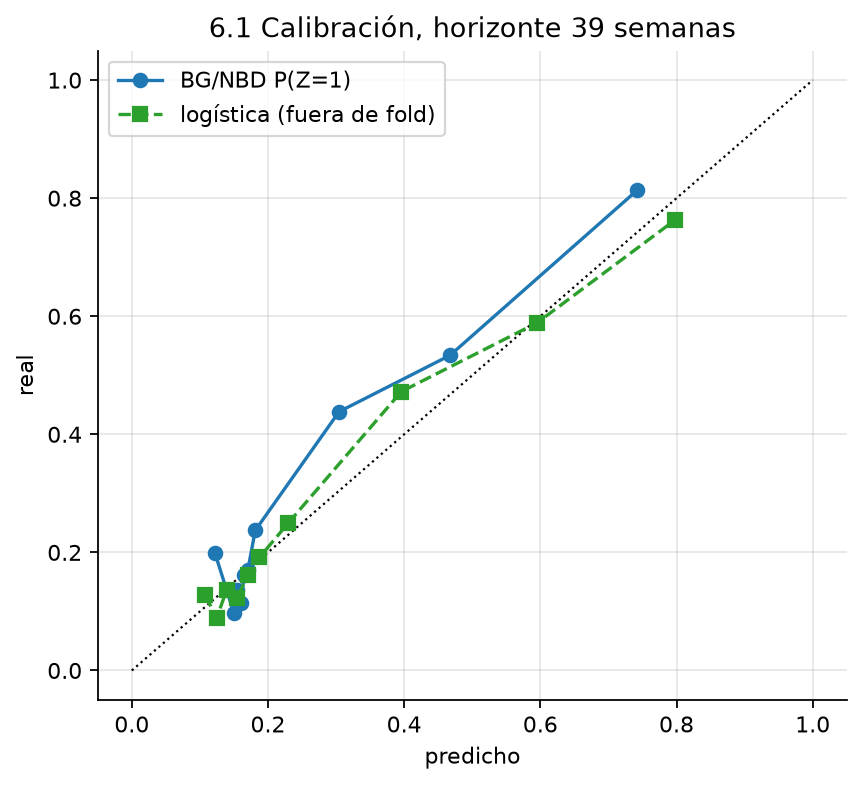
\includegraphics[width=\linewidth]{6_1_calibracion}
\column{0.58\textwidth}\small
CV 5 \emph{folds} $\times$ 20 semillas:\\
\begin{tabular}{lrr}\toprule
 & AUC & Brier\\\midrule
Logística & 0.779 & 0.156\\
BG/NBD & 0.757 & 0.161\\\bottomrule
\end{tabular}\\[0.3em]
Coeficientes: $t_x$ +0.80, $x$ +0.47, $T$ $-0.23$.\\[0.3em]
\alert{Fuga}: aprendió con etiquetas del \emph{holdout} de esta misma cohorte. El 30-sep-1997 esas etiquetas no existían; igual que la validación cruzada aleatoria en series de tiempo.
\end{columns}
\end{frame}

\begin{frame}{6.3–6.4 La versión honesta y cambiar de horizonte}
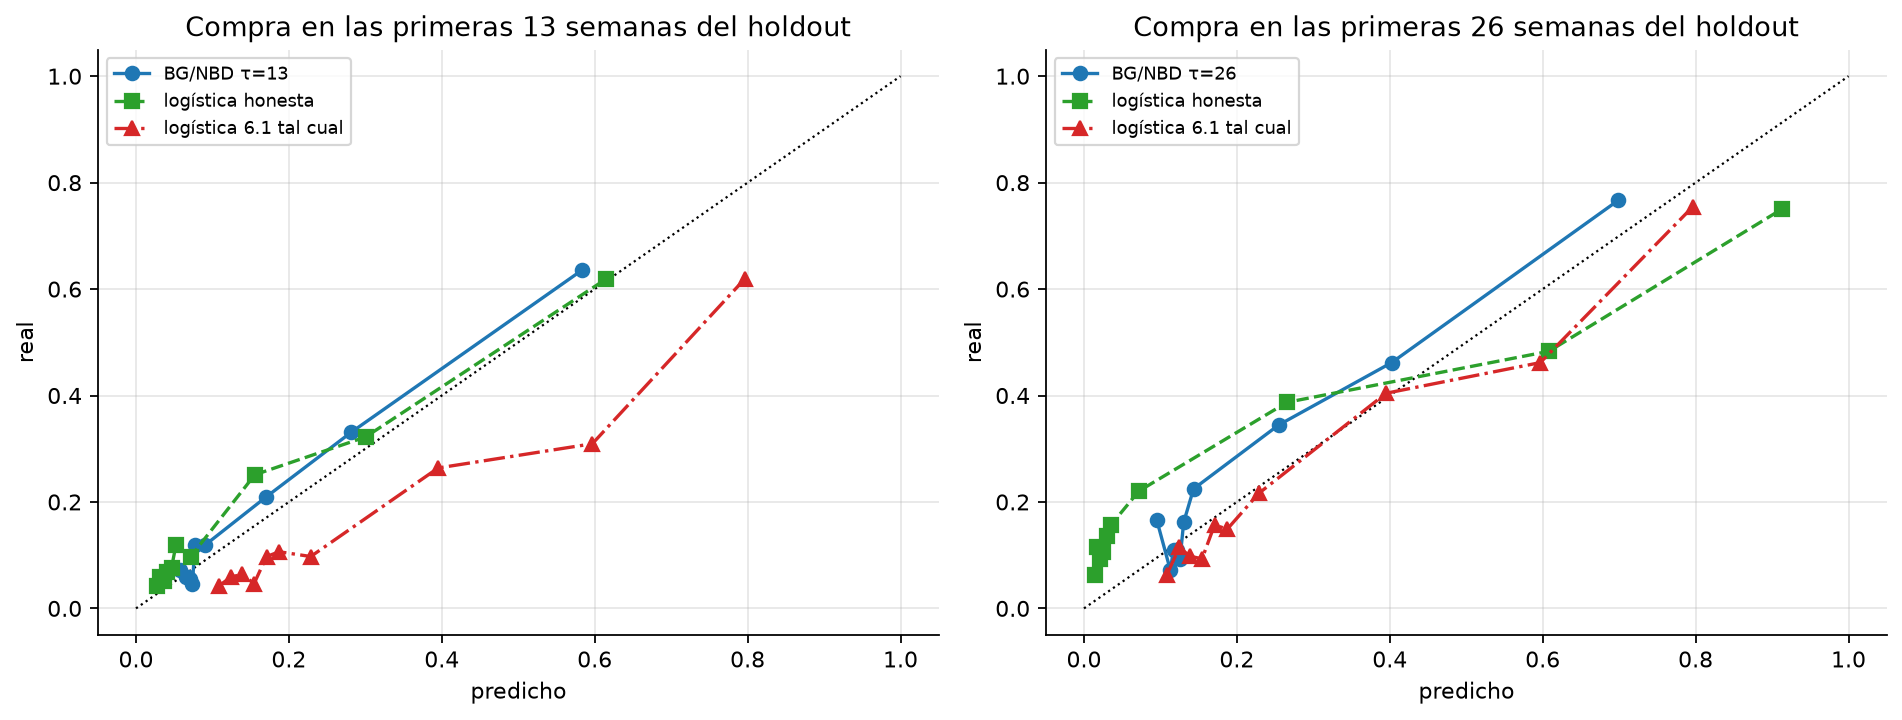
\includegraphics[width=0.6\linewidth]{6_3_6_4_calibracion}\hfill
\begin{minipage}[b]{0.36\linewidth}\scriptsize
\begin{tabular}{lrr}\toprule
13 sem (real 17.1\%) & AUC & Brier\\\midrule
Logística honesta & 0.792 & 0.112\\
BG/NBD $\tau=13$ & 0.785 & \alert{0.110}\\
Logística 6.1 & 0.791 & 0.128\\\midrule
26 sem (real 25.1\%) & & \\\midrule
Logística honesta & 0.785 & 0.156\\
BG/NBD $\tau=26$ & 0.762 & \alert{0.148}\\\bottomrule
\end{tabular}\\[0.3em]
La logística honesta \alert{extrapola}: se entrena con $T\in[14,26]$ y se aplica a $T\in[27,39]$. La de 6.1 usada a 13 semanas promedia 29\% cuando la tasa es 17\%.
\end{minipage}
\end{frame}

\begin{frame}{6.5 Veredicto}
\begin{columns}[T]
\column{0.5\textwidth}
\textbf{Logística}
\begin{itemize}\small
  \item Pregunta fija, mismo horizonte, sobre todo \emph{ordenar}.
  \item Hay etiquetas de un periodo anterior comparable.
  \item Se quieren más variables (monto, canal\ldots).
\end{itemize}
\column{0.5\textwidth}
\textbf{BG/NBD}
\begin{itemize}\small
  \item Se necesitan \emph{niveles}: cuántos compran, cuántas compras, CLV.
  \item Horizonte variable sin reentrenar.
  \item Total de la base \emph{bottom-up}.
  \item \alert{No hay etiquetas} del pasado (cohorte nueva).
\end{itemize}
\end{columns}
\vspace{1em}
Lo mejor de los dos: usar $P(Z=1)$ y $E[Y(\tau)]$ del BG/NBD como variables de la logística.
\end{frame}

\begin{frame}{Conclusiones}
\begin{enumerate}\small
  \item Verosimilitud a mano validada: recupera parámetros simulados y reproduce el artículo (estimados, $-4\%$ acumulado, condicionales, $\rho=0.626$).
  \item Bottom-up le gana a casi todo top-down sin escoger ventanas: sabe que la cohorte está cerrada.
  \item \alert{``Vivo'' $\neq$ ``va a comprar''}: $\pvivo=1$ para $x=0$ es un artefacto del supuesto de muerte; $P(Z=1)$ es la pregunta correcta.
  \item El BG/NBD es una elección: en Online Retail la muerte desaparece y la falta de estacionalidad cuesta 38\% en noviembre.
  \item La logística solo ``gana'' si ve el futuro.
\end{enumerate}
\vspace{0.5em}
\centering\small Código: notebook \texttt{proyecto2.ipynb} + paquete \texttt{btyd/} (todo a mano con \texttt{scipy}).
\end{frame}

\end{document}
